\documentclass[12pt]{article}
\usepackage{fullpage}
\usepackage{graphicx}
\usepackage{xcolor}
\definecolor{TSIBlack}{HTML}{040404}
\begin{document}
\pagecolor{TSIBlack}
\color{white}
\begin{titlepage}
\begin{center}
\huge GAME MACHINE
\end{center}
\begin{center}
 BY
\end{center}
\begin{center}
\huge Tiny Shark Interactive
\end{center}
\begin{center}

\includegraphics[scale=0.6]{banner.png}
\end{center}
\end{titlepage}
\tableofcontents
\pagebreak
\section{Introduction}
This Game Machine is a plugin for unreal engine 4.10 and above.
We have designed this plugin for designing mission.
\section{General description}
\section{Specific requirements}
\section{Overview}
\section{How to use}
	  \subsection{overview}
	  In game machine there are two type of graphs mission graph and dialogue graph which will going to give help mission designers to design missions easy and more afficent way.   
	  \subsection{Mission Graph}
	  Mission Graph is the place where we are going to define the flow of our mission and design objectives.
	  Here in mission graph there are four node's Mission-Root-Node, Objective-Node,Branched-Objective-Node,Multi-Objective-Node
	  \begin{center}
	  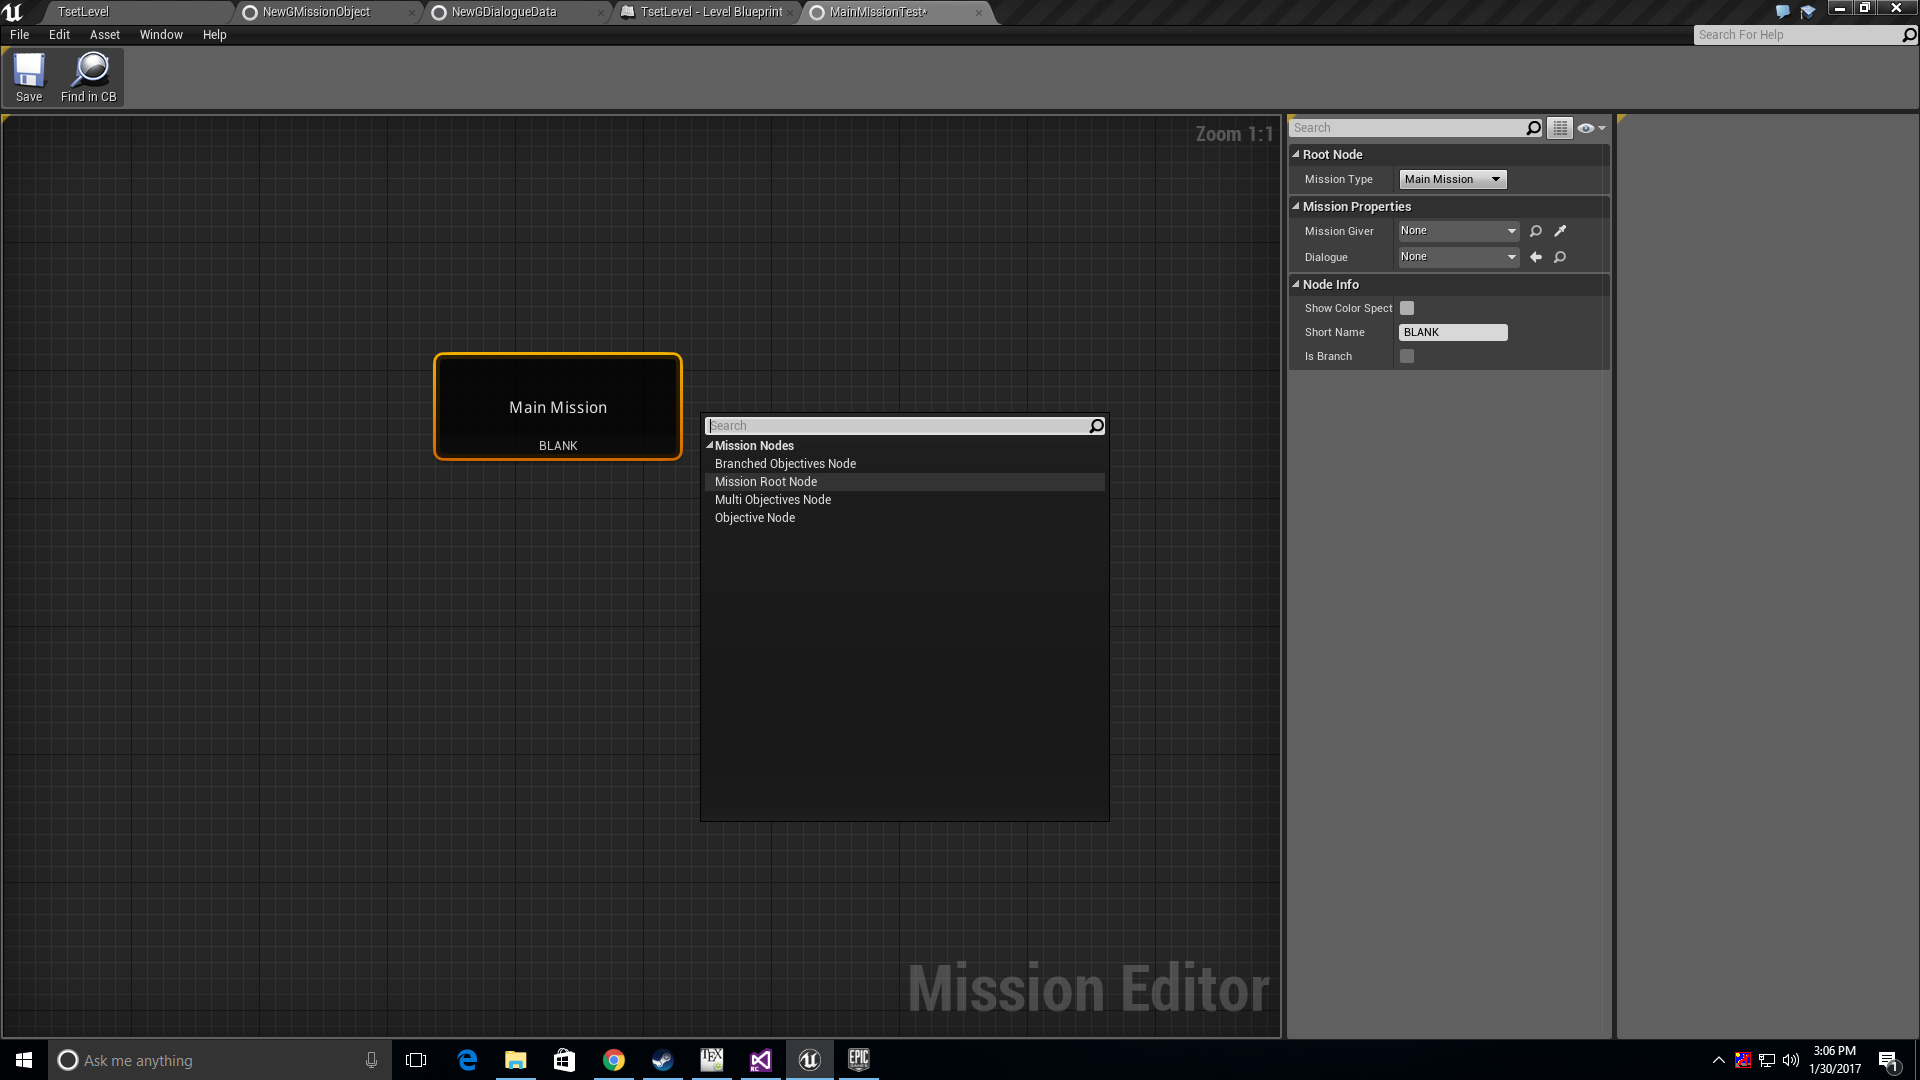
\includegraphics[scale=0.2]{MissionRootNode.png}
	  \end{center}
	  \begin{center}
	  \textit{MISSION ROOT NODE}\\
	  --------------------------------------
	  \end{center}
	  This is the entry node from where our mission will be initialized.
	  \begin{center}
	  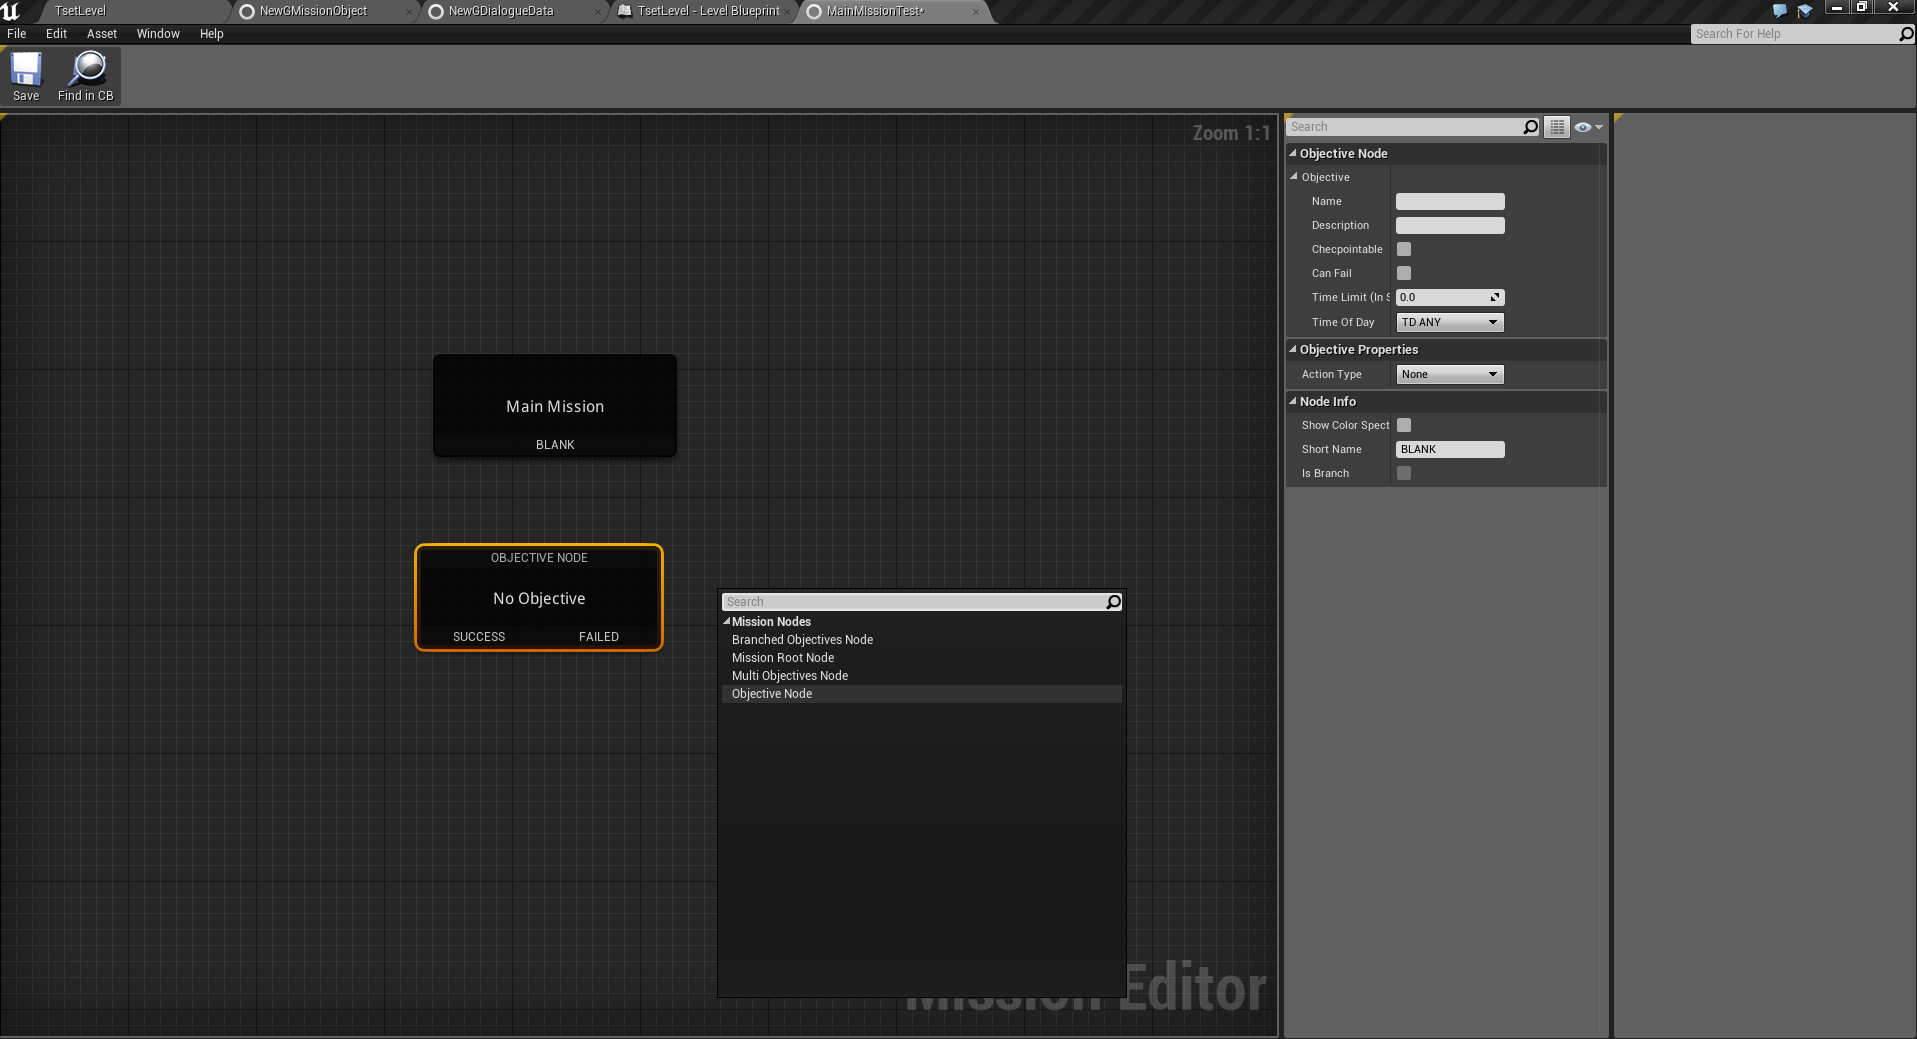
\includegraphics[scale=0.2]{ObjectiveNode.png}
	  \end{center}
	  \begin{center}
	  \textit{OBJECTIVE NODE}\\
	  \----------------------------------
	  \end{center}
	  This is the node where we design our objective.
	   \begin{center}
	  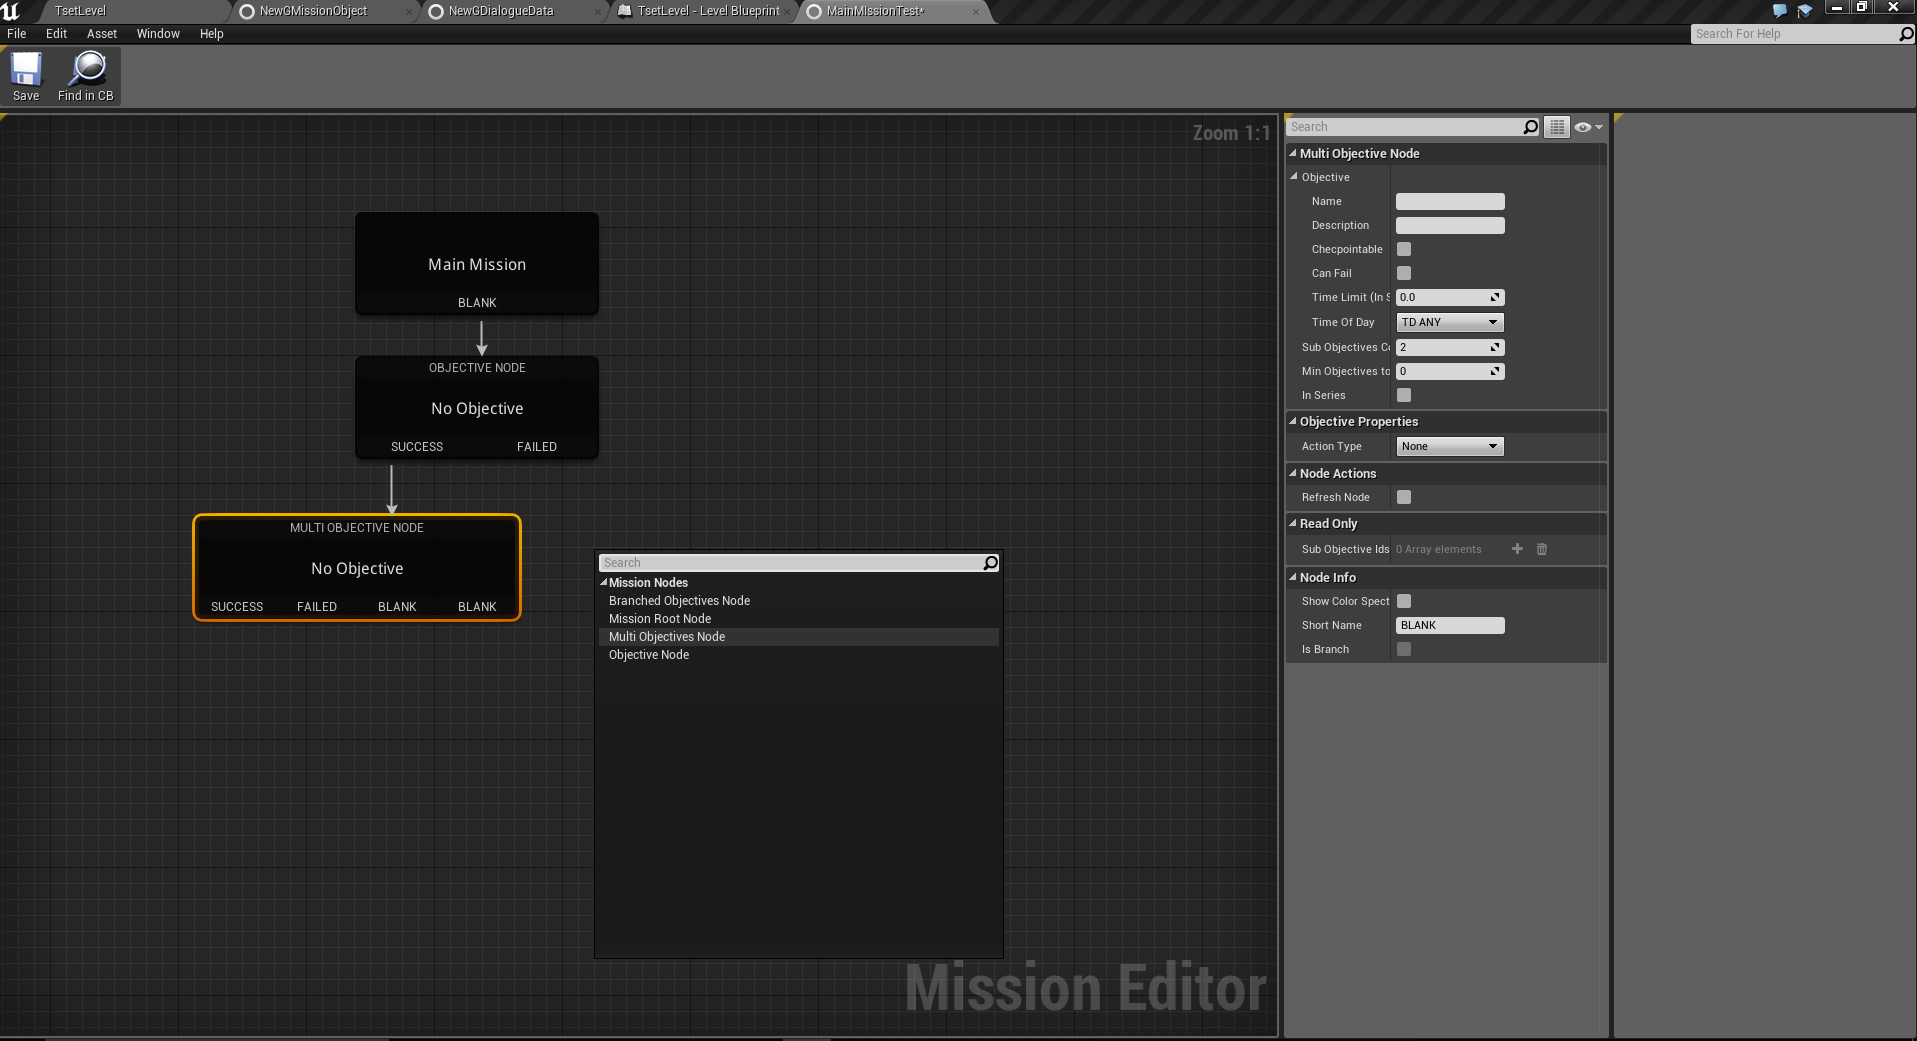
\includegraphics[scale=0.2]{MultiObjectiveNode.png}
	  \end{center}
	  \begin{center}
	  \textit{MULTI OBJECTIVE NODE}\\
	  \----------------------------------
	  \end{center}
	  This node same as an objective node but in this node we can design an objective which can have multiple objective.hsajdja asjdsa sajh sad hjsa hjksad ajhd as sh as sa h
	  a usa uhsa hsa hsad hsaj sajhsda jsa sai gisa dsagh id iuasd hisda asd giasd iuasdhsa hid hiuasduih iuasd\\
	  asd jisa joasd oiasdiod iojsa
	   \begin{center}
	  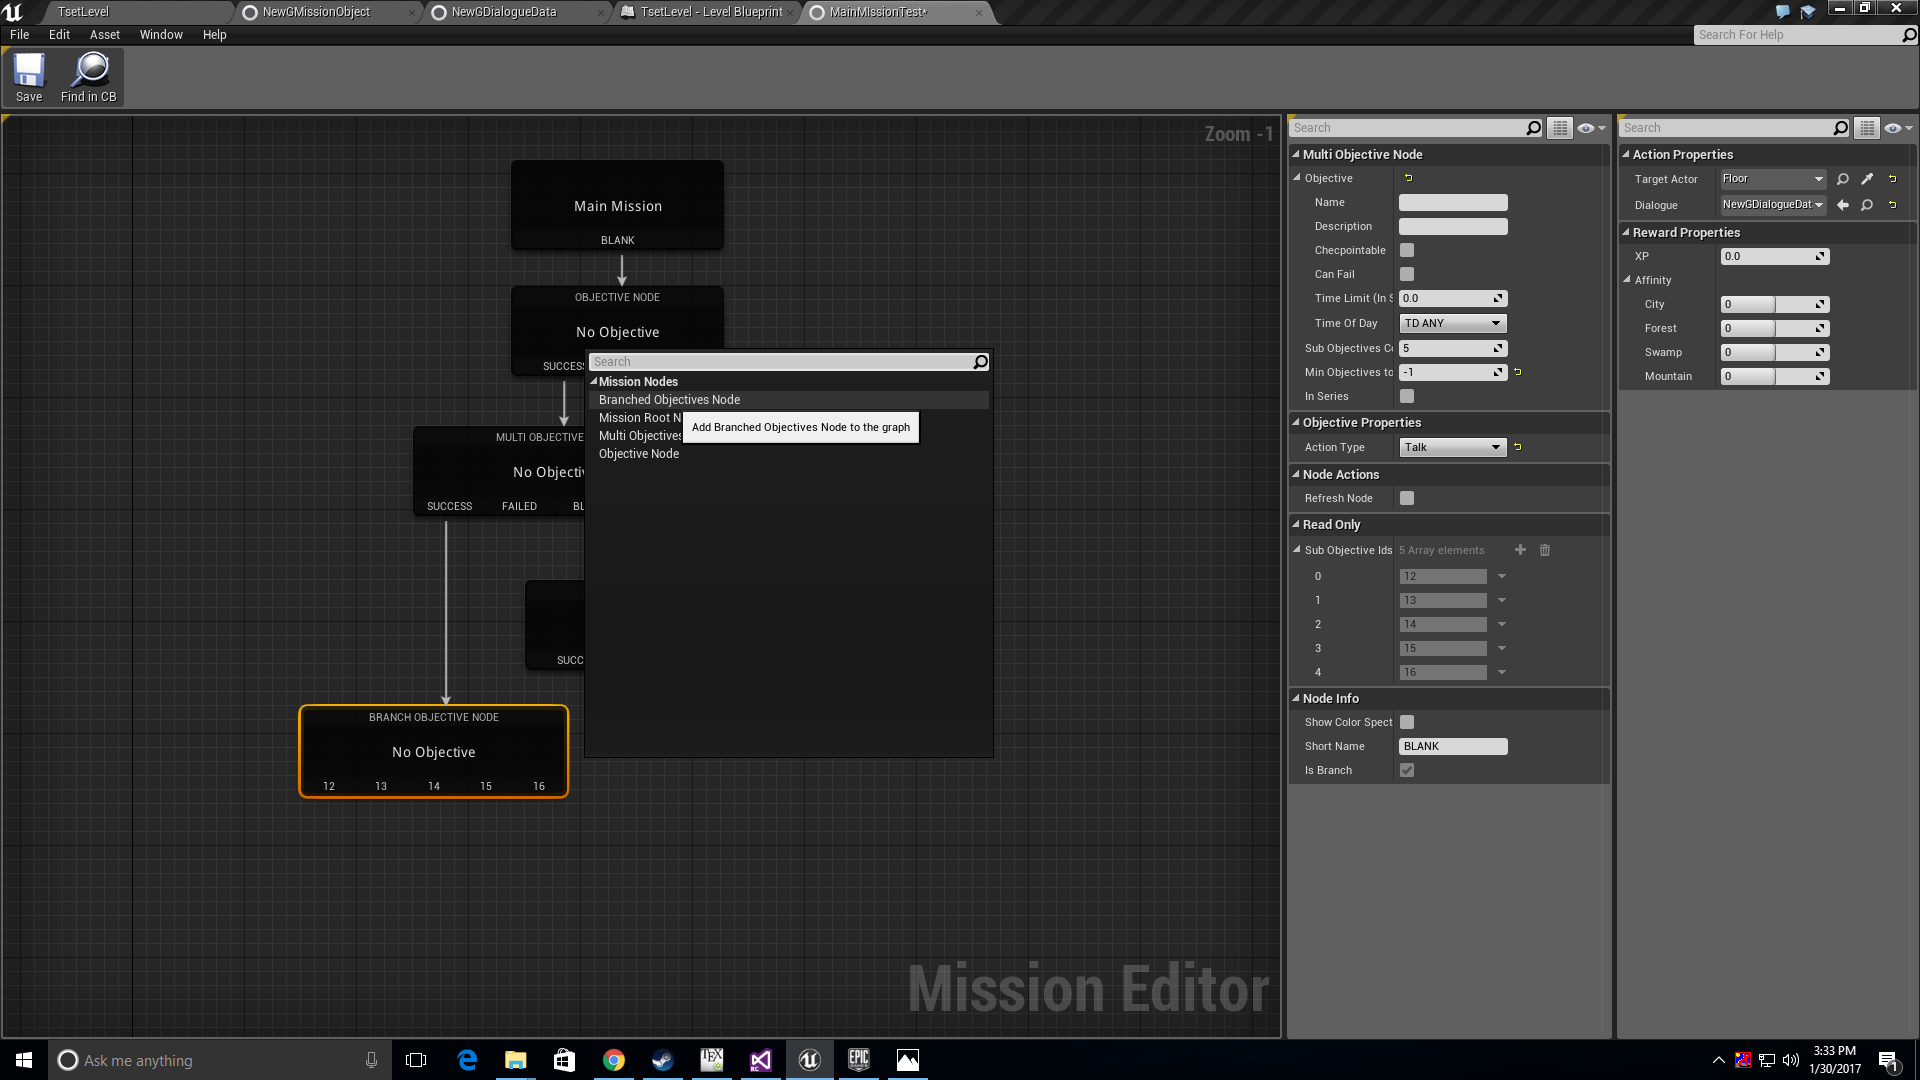
\includegraphics[scale=0.2]{BranchedObjectiveNode.png}
	  \end{center}
	  \begin{center}
	  \textit{BRANCHED OBJECTIVE NODE}\\
	  \---------------------------------------------- 
	  \end{center}
	  	  Branched Objective Node is the similar to the Multi Objective Node With slight difference.\\
	  \subsubsection{MISSION ROOT NODE}
	  As we know Mission root node is the initialization node which initialize our mission graph, this node have few properties.\\
	  \begin{center}
	 	 \begin{tabular}{|c|c|}\hline
			Properties Name(Section) & Properties Description\\					\hline\hline
			Mission Type(Root Node) & Main Mission : for main 					missions\\& Side Mission : for side missions\\\hline
			Mission Giver(Mission Properties) & Actor which is 					going to give mission \\ & or actor form where 						mission is going to start\\\hline
			Show Color Spectrum(Node Info) & show the nodes 					color\\\hline
			Short Name(Node Info) & Name of the node\\\hline
			IsBranch(Node Info) & if node is branched\\\hline
			
			
		\end{tabular}
	  \end{center}
	\pagebreak
	  \subsubsection{OBJECTIVE NODE}
	  this is the node where we describe our missions objective.\\
	  Details Panel:-
	  	\begin{center}
	  		\begin{tabular}{|c|c|}\hline
				Properties Name(Section)&Properties Description\\\hline\hline	 Name(Objective Node) & Name of the objective\\\hline
				Description(Objective Node)& What mission is about\\\hline
				Checkpointable(Objective Node)& Is objective is having check point or not\\\hline
				Can Fail(Objective Node) & Objective can fail or not\\\hline
				Time Limit(Objective Node) & Is an Objective having any time limits or not and time\\ 
				&is in seconds\\\hline
				Time Of Day(Objective Node) & In which time objective will be accessible\\
				& (Morning,Noon,Evening,Night)\\\hline
				Action Type(Objective Properties)& Action type of the objective\\\hline
					Show Color Spectrum(Node Info) & show the nodes 					color\\\hline
			Short Name(Node Info) & Name of the node\\\hline
			IsBranch(Node Info) & if node is branched\\\hline				
	  		\end{tabular}\\
	  	\end{center}
	  		Action Panel:-	
	  \begin{center}
	  	\begin{tabular}{|c|c|}\hline
	  	Properties Name(Section)& Properties Description\\\hline\hline
	  	Location(Action Properties)&Location of the actor which is going to perform action\\\hline
	  	Radius(Action Properties)& Radius is the distance according to which action going to execute\\\hline 
	  	XP(Reward Properties)& hsjdfhksdjhfkjshdfkj\\\hline
	  	Affinity(Reward Properties)& In affinity there are four option which can be manipulated.\\
	  	& (City,Forest,Swamp,Mountain)\\\hline
	  		  		
	  	\end{tabular}
	  \end{center}
	  \pagebreak
	  \subsubsection{MULTI OBJECTIVE NODE}
	  This is an objective node which can contain multiple objective.\\
	  Details Panel:-
	  \begin{center}
	  	\begin{tabular}{|c|c|}\hline
	  	Properties Name(Section)& Properties Description\\\hline\hline
	  	Name(MultiObjectiveNode)& Name of the objective\\\hline
	  	Description(MultiObjectiveNode)& Description about the objective\\\hline
	  	Checkpointable(MultiObjectiveNode)& is the objective have check points or not\\\hline
	  	CanFail(MultiObjectiveNode)& is objective can fail or not\\\hline
	  	TimeLimit(MultiObjectiveNode)& is the objective have time limit or not\\
	  	& and the time limit is in second's	\\\hline
	  	TimeOfDay(MultiObjectiveNode)& In which time of the day objective can be done \\\hline
	  	SubObjectiveCount(MultiObjectiveNode)&How many sub objective are in this objective node\\\hline
	  	MinObjectivesToComplete(MultiObjectiveNode)&What is the min no. of objective in total\\
	  	& have to be done to complete this objective\\\hline
	  	InSeries(MultiObjectiveNode)& is the objective have to be done in series \\
	  	&or not\\\hline
	  	ActionType(ObjectiveProperties)&Type of the action which this objective is \\
	  	& going to perform\\\hline
	  	RefresNode(NodeAction)& For refreshing the multi objective node after\\
	  	& selecting the action type\\\hline
	  	SubObjectiveIDs(ReadOnly)&\\\hline
	  						Show Color Spectrum(Node Info) & show the nodes 					color\\\hline
			Short Name(Node Info) & Name of the node\\\hline
			IsBranch(Node Info) & if node is branched\\\hline
	  	
	  	\end{tabular}
	  \end{center}
	  If Action Type(Objective Properties) is Move to.\\
	  Action Panel:-
	  \begin{center}
	  	\begin{tabular}{|c|c|}\hline
	  	Properties Name(Section)& Properties Description\\\hline\hline
	  	Location(ActionProperties) & Location of the actor where to move\\\hline
	  	Radius(ActionProperties) & radius is the distance in which an event is going to activate\\\hline
	  		  	XP(Reward Properties)& hsjdfhksdjhfkjshdfkj\\\hline
	  	Affinity(Reward Properties)& In affinity there are four option which can be manipulated.\\
	  	& (City,Forest,Swamp,Mountain)\\\hline
	  	\end{tabular}
	  \end{center}
	  \pagebreak
	    If Action Type(Objective Properties) is Talk.\\
	  Action Panel:-
	  \begin{center}
	  	\begin{tabular}{|c|c|}\hline
	  	Properties Name(Section)& Properties Description\\\hline\hline
	  	TargetActor(ActionProperties) & Actor which is going to speek\\\hline
	  	Dialogue(ActionProperties) & dialogue of the target actor\\\hline
	  		  	XP(Reward Properties)& hsjdfhksdjhfkjshdfkj\\\hline
	  	Affinity(Reward Properties)& In affinity there are four option which can be manipulated.\\
	  	& (City,Forest,Swamp,Mountain)\\\hline
	  	\end{tabular}
	  \end{center}
	    If Action Type(Objective Properties) is Mind Voice.\\
	  Action Panel:-
	  \begin{center}
	  	\begin{tabular}{|c|c|}\hline
	  	Properties Name(Section)& Properties Description\\\hline\hline
	  	Dialogue(ActionProperties) & Character's dialogue\\\hline
	  		  	XP(Reward Properties)& hsjdfhksdjhfkjshdfkj\\\hline
	  	Affinity(Reward Properties)& In affinity there are four option which can be manipulated.\\
	  	& (City,Forest,Swamp,Mountain)\\\hline
	  	\end{tabular}
	  \end{center}
	  \pagebreak
	  \subsubsection{BRANCHED OBJECTIVE NODE}
 Branched Objective Node is the similar to the Multi Objective Node With slight difference.\\
	  Details Panel:-
	  \begin{center}
	  	\begin{tabular}{|c|c|}\hline
	  	Properties Name(Section)& Properties Description\\\hline\hline
	  	Name(MultiObjectiveNode)& Name of the objective\\\hline
	  	Description(MultiObjectiveNode)& Description about the objective\\\hline
	  	Checkpointable(MultiObjectiveNode)& is the objective have check points or not\\\hline
	  	CanFail(MultiObjectiveNode)& is objective can fail or not\\\hline
	  	TimeLimit(MultiObjectiveNode)& is the objective have time limit or not\\
	  	& and the time limit is in second's	\\\hline
	  	TimeOfDay(MultiObjectiveNode)& In which time of the day objective can be done \\\hline
	  	SubObjectiveCount(MultiObjectiveNode)&How many sub objective are in this objective node\\\hline
	  	MinObjectivesToComplete(MultiObjectiveNode)&What is the min no. of objective in total\\
	  	& have to be done to complete this objective\\\hline
	  	InSeries(MultiObjectiveNode)& is the objective have to be done in series \\
	  	&or not\\\hline
	  	ActionType(ObjectiveProperties)&Type of the action which this objective is \\
	  	& going to perform\\\hline
	  	RefresNode(NodeAction)& For refreshing the multi objective node after\\
	  	& selecting the action type\\\hline
	  	SubObjectiveIDs(ReadOnly)&\\\hline
	  						Show Color Spectrum(Node Info) & show the nodes 					color\\\hline
			Short Name(Node Info) & Name of the node\\\hline
			IsBranch(Node Info) & if node is branched\\\hline
	  	
	  	\end{tabular}
	  \end{center}
	  If Action Type(Objective Properties) is Move to.\\
	  Action Panel:-
	  \begin{center}
	  	\begin{tabular}{|c|c|}\hline
	  	Properties Name(Section)& Properties Description\\\hline\hline
	  	Location(ActionProperties) & Location of the actor where to move\\\hline
	  	Radius(ActionProperties) & radius is the distance in which an event is going to activate\\\hline
	  		  	XP(Reward Properties)& hsjdfhksdjhfkjshdfkj\\\hline
	  	Affinity(Reward Properties)& In affinity there are four option which can be manipulated.\\
	  	& (City,Forest,Swamp,Mountain)\\\hline
	  	\end{tabular}
	  \end{center}
	  \pagebreak
	    If Action Type(Objective Properties) is Talk.\\
	  Action Panel:-
	  \begin{center}
	  	\begin{tabular}{|c|c|}\hline
	  	Properties Name(Section)& Properties Description\\\hline\hline
	  	TargetActor(ActionProperties) & Actor which is going to speek\\\hline
	  	Dialogue(ActionProperties) & dialogue of the target actor\\\hline
	  		  	XP(Reward Properties)& hsjdfhksdjhfkjshdfkj\\\hline
	  	Affinity(Reward Properties)& In affinity there are four option which can be manipulated.\\
	  	& (City,Forest,Swamp,Mountain)\\\hline
	  	\end{tabular}
	  \end{center}
	    If Action Type(Objective Properties) is Mind Voice.\\
	  Action Panel:-
	  \begin{center}
	  	\begin{tabular}{|c|c|}\hline
	  	Properties Name(Section)& Properties Description\\\hline\hline
	  	Dialogue(ActionProperties) & Character's dialogue\\\hline
	  		  	XP(Reward Properties)& hsjdfhksdjhfkjshdfkj\\\hline
	  	Affinity(Reward Properties)& In affinity there are four option which can be manipulated.\\
	  	& (City,Forest,Swamp,Mountain)\\\hline
	  	\end{tabular}
	  \end{center}
	  \subsection{Dialogue Graph}
	  Now in Dialogue graph we are going to design our dialogue's as per the mission graph.
	  \subsubsection{DIALOGUE ROOT NODE}
	  \subsubsection{DIALOGUE NODE}
	  \subsubsection{BRANCH NODE}
	  \subsubsection{END NODE}
	  \section{Examples}
	  \section{Appendix}
\end{document}